\documentclass{article}
\usepackage{graphicx} % new way of doing eps files
\usepackage{listings} % nice code layout
\usepackage[usenames]{color} % color
\definecolor{listinggray}{gray}{0.9}
\definecolor{graphgray}{gray}{0.7}
\definecolor{ans}{rgb}{1,0,0}
\definecolor{blue}{rgb}{0,0,1}
% \Verilog{title}{label}{file}
\newcommand{\Verilog}[3]{
  \lstset{language=Verilog}
  \lstset{backgroundcolor=\color{listinggray},rulecolor=\color{blue}}
  \lstset{linewidth=\textwidth}
  \lstset{commentstyle=\textit, stringstyle=\upshape,showspaces=false}
  \lstset{frame=tb}
  \lstinputlisting[caption={#1},label={#2}]{#3}
}


\author{Matthew Carrano and Breana Leal}
\title{Lab 3}

\begin{document}
\maketitle

\section{Introduction}
The goal of this lab is to create an instruction memory module and combine previous modules to form the fetch stage, iFetch.  The instruction memory  will be used to store instructions. The instruction memory reads in data from the program counter that requires addressing executable instructions. The fetch stage is the first stage in building the ARM computer that combines the previous labs. The fetch stage will be followed by the decode stage.

\section{Interface}
The inputs of the instruction memory module are clk and pc. The clk is initiated to follow a positive clock edge. With each cycle, pc will increment which should give a value for its output instruction to address from a memory file.  
The inputs of the iFetch are clk, reset, pc\_src, and branch\_target. The output of the iFetch is incremented\_pc, instruction, and cur\_pc. Its inputs and outputs serve as connecting pieces for the previously discussed modules mux, register, adder, and instruction memory.

incremented\_pc and branch\_target are the two signals that are available to be selected, and pc\_src is the signal that is used to select whether the value of incremented\_pc or branch\_target will be chosen by the mux. new\_pc is a wire that contains the value that the mux selected. The output from the mux becomes an input for the register along with inputs clk and reset. The output for the register becomes cur\_pc. Similarly, cur\_pc becomes an input for the adder module. The adder's other input is STEP, a parameter defined as 'WORD'd4 and its output is incremented\_pc. Finally, the instru\_mem module has inputs clk and cur\_pc. The cur\_pc is the current program counter value and notifies ARM about the current instruction address. The output instruction is the final data from the provided memory file. 

As noted, the fetch stage connects the previous modules in having one's input become another's output and reiterate the process to continuously update the instruction results either sequentially or branching.
\section{Design}
The first module to build is the instruction memory module.  The instruction memory module is designed to take one 64-bit input value and produce a 32-bit data from a readable file as an output.

The second module to build is the iFetch module.  The iFetch module is designed to process five input values with four individually instantiated modules (discussed in Interface). Each module processes its own inputs to has its own output that work under the iFetch module to evaluate the final instruction value for the fetch stage to pass onto the decode stage. 
\section{Implementation}
The instruction memory module is implemented by having a 32-bit data reg imem. The output instruction is set to equal the program counter divided by 4 indexed data. Meaning, the instruction should equal the adjusted 32 bit data read from the file. For example, if the program counter is set to 8, the instruction will out put the binary code, line 2, from the readable file. This is done continuously and updated with each input change.
\Verilog{Verilog code for implementing the instruction memory module.}{code:adder}{../code/1_fetch/instr_mem.v}

The iFetch module is implemented instantiating the mux, register, adder, and instruction memory modules. The instantiations easily verify the connections the fetch stage makes. 

mux is altered to have a WORD parameter and instruction memory SIZE parameter for future reference purposes. 
\Verilog{Verilog code for implementing the iFetch module.}{code:mux}{../code/1_fetch/iFetch.v}
\section{Test Bench Design}
A test bench was made for each module. The instruction memory test bench creates a wire for the input clock (clk), and 32 bit wire for the instruction output (inst). A 64 bit reg is created for the program counter input (p\_c). An oscillator module called clock\_gen is instantiated. This generates a clock pulse on clk. An instruction memory module called UUT is then instantiated. In the initial section the p\_c is set from 0 to 52 with increments of 4 and delays of 1 cycle (10ns) in between each increment. This simulates the incrementation of the program counter by the adder in the fetch stage. The instruction data used for testing is shown in Figure ? with the decimal values to the right of each binary value. Only the binary values were present at testing. The results of the test are verified if the output of the module (inst) is the value at the address specified by the p\_c. For example, at p\_c equal to 0, the output should be 4165927241 because this is the data at the 0 address of the test data file. All of the code used for the instruction memory testing is in Listing~\ref{code:instrtest}.
\Verilog{Verilog code for testing the fetch stage.}{code:instrtest}{../code/1_fetch/instr_mem_test.v} 

Next, a test bench was created for the fetch module. This required the creation of a wire called clk, a rst and pc\_s reg, a 64 bit branch reg, a 64 bit inc\_pc wire, a 32 bit instr wire, and a 64 bit c\_pc wire. Another oscillator module was instantiated, and then a iFetch module called UUT was also instantiated. To test functionality, first, the pc\_s was set with a blocking statement to 0 in order to perform sequential stepping. The reset reg is set to 0 with a non-blocking statement. This set the program counter to an initial value of 0. Then a delay of 4 cycles occurs. With these three lines of code we can verify that the sequential fetching works correctly. In the simulation we should see the program counter start at 0 and increment by 4. As this is happening the respective instructions should be outputted (the same instruction data was used). After the 4 cycles are finished the pc\_s is set to 1 and the branch is set to 4. A delay of 2 cycles is added. This is used to verify that the branching functionality works. We should see the program counter change to 4 at a positive clock edge, and then stay at 4 until the pc\_s is set back to 0. When p\_c is set back to 0, the program counter will resume stepping by 4 starting with the branch value. All of the code used for the iFetch testing is in Listing~\ref{code:fetchtest}.

\Verilog{Verilog code for testing the fetch stage.}{code:fetchtest}{../code/1_fetch/iFetch_test.v}

\section{Simulation}
The timing diagrams in Figure 2 and 3 verify that both modules work as detailed in the above section.

\begin{center}
	\caption{Figure 2. Timing diagram for instruction module test.}\label{fig:instrmemtest}
	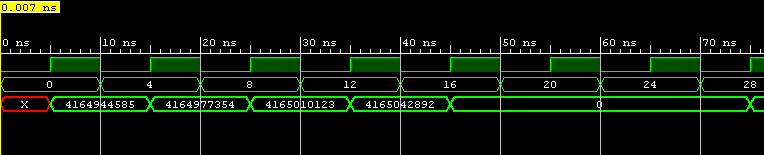
\includegraphics[width=1\textwidth]{../images/instr_memSim1.png}
\end{center}

\begin{center}
\caption{Figure 3. Timing diagram for fetch module test.}\label{fig:fetchtest}
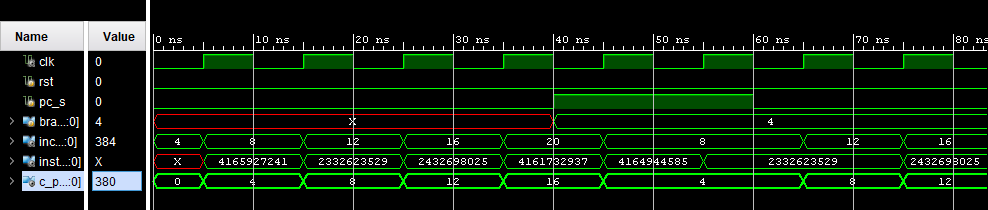
\includegraphics[width=1\textwidth]{../images/fetch_sim.png}
\end{center}


\section{Conclusions}
The instruction module and fetch stage were successfully established.  The instruction memory module is used in conjunction with the mux, register, and adder modules. The instruction memory is established to gather data from a file based on addressed instruction values from the program counter. Combined, these modules form the first stage for the ARM-64 that will be further processes in the decoding stage.
\end{document} 